\section{Approach}
\label{sect:approach}
\subsection{Overview}
\reffig{architecture} shows the high-level architecture of our system.
\begin{figure}[htb]
\centering
\includegraphics[width=0.5\textwidth]{arch}
\caption{}
\label{fig:architecture}
\end{figure}

\subsection{Configuration Module}
In the configuration file, users only need to configure 3 parameters for a services. The following figure is part of a configuration file.
The minimum rate parameter specifies the minimum bandwidth the service requires.The recommended rate parameter specifies the desired bandwidth for the service.
The priority parameter specifies the users' prefenrece for the service.
For example, in the figure, the minimum rate for video is 1.5M and the recommended rate for vidoe is 7M. The priority for video, which is 10, is much higher than other types of services. So our SDN controller will try to first satisfy the QoS requirements for the video services in the network.

User define configuration in YAML format
\subsection{Flow classfier module}
Static flow classifier
\subsection{Traffic monitor module}
\begin{itemize}
\item Flow statistics
\item Port statistics
\end{itemize}
\subsection{Control Module}
On a high level, our control module tries to satisfy a maximum number of QoS requirements with the limited bandwidth.
Each type of service has been configured by the user with a priority. We assign a weight to the service based on the actual bandwidth it will get. For example, the weight of a service is 0.6 if the minimum rate bandwidth is achieved. The weight is 1.0 if the recommended rate bandwidth is achieved.
Our algorithm allocates bandwidth to different services to get the maximum value of $$\sum_{i=1}^{n} Weight_i*Prioriy_i $$ under the condition that
$$\sum_{i=1}^{n} Bandwidth_i <= C $$. C is the total bandwidth of the network.


\subsubsection{Dynamic queue assignment algorithm}

\begin{figure}[htb]
\centering
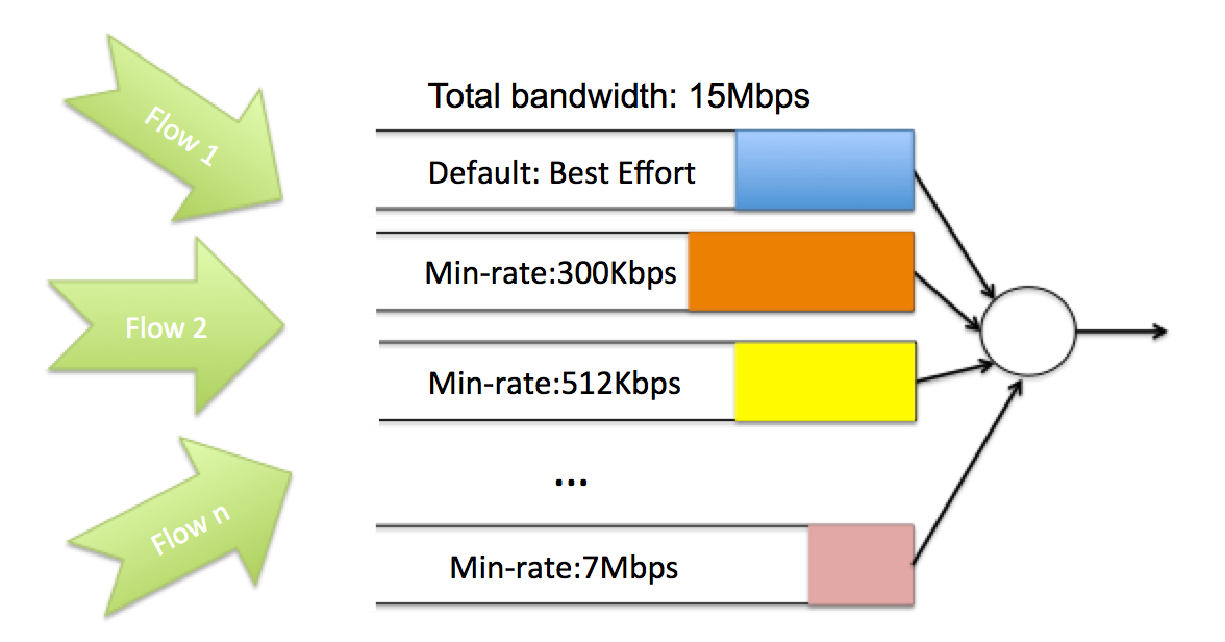
\includegraphics[width=0.5\textwidth]{assign_queue}
\caption{}
\label{fig:assign_queue}
\end{figure}

\subsection{Web Portal Module}
This module is for user configuration and traffic statistics.
\subsection{Implementation}
Implementation is based on Ryu SDN controller~\cite{ryu} and OpenVSwitch.
